% Chapter Template

\chapter{Ensayos y resultados} % Main chapter title

\label{Chapter4} % Change X to a consecutive number; for referencing this chapter elsewhere, use \ref{ChapterX}

En este capítulo se detallan las pruebas unitarias realizadas al \textit{frontend} y \textit{backend} y la prueba de integración del sistema completo.

%----------------------------------------------------------------------------------------
%	SECTION 1
%----------------------------------------------------------------------------------------

\section{Pruebas del \emph{frontend}}

Para probar el \textit{frontend} se decidió utilizar una batería de pruebas unitarias \citep{WEBSITE:UNITTESTING} creadas con Jasmine y Karma. Estás fueron completamente automatizadas para garantizar y asegurar la calidad de código. Se realizaron 208 pruebas unitarias para lograr un 100\% de cobertura de código.

En la figura \ref{fig:unitTestingFrontend} se visualiza el proceso de ejecución de las pruebas unitarias con Karma.

\begin{figure}[H]
	\centering
	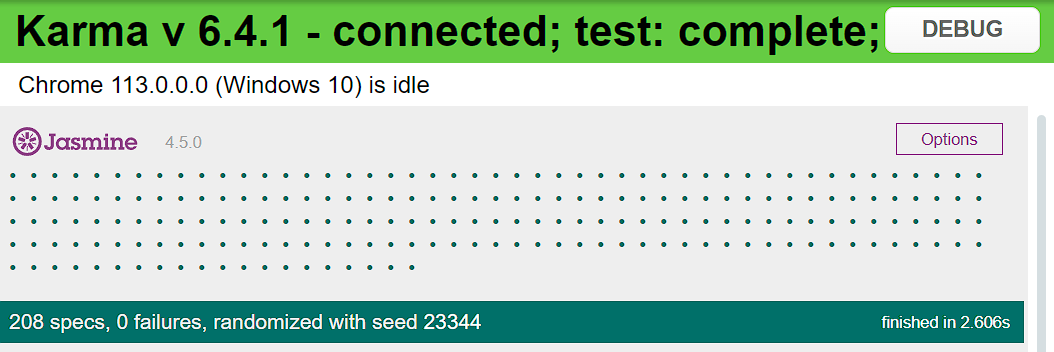
\includegraphics[width=.9\textwidth]{./Figures/Frontend unit testing.png}
	\caption{Pruebas unitarias.}
	\label{fig:unitTestingFrontend}
\end{figure}

En la figura \ref{fig:codeCoverageFrontend} se visualiza la cobertura de código del \emph{frontend}.

\begin{figure}[H]
	\centering
	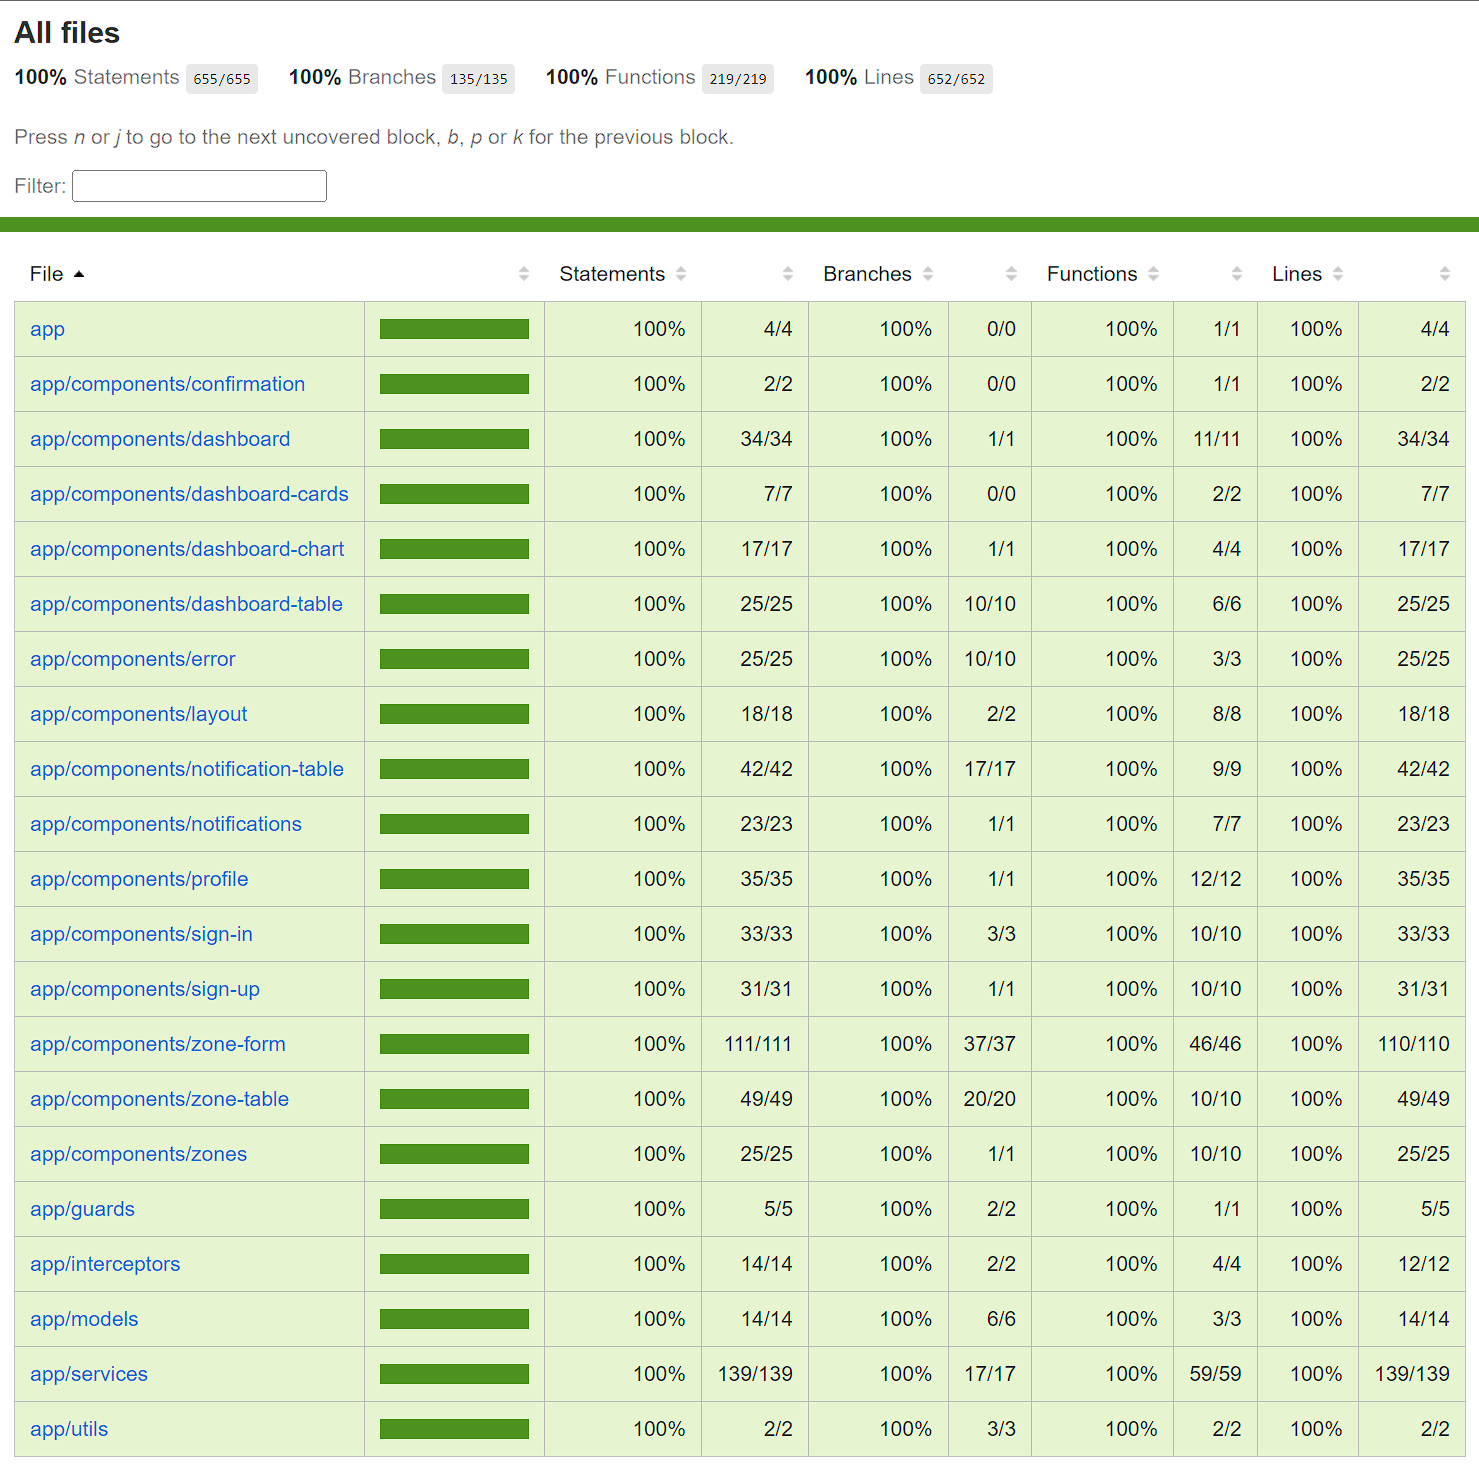
\includegraphics[width=.9\textwidth]{./Figures/Frontend code coverage.png}
	\caption{Cobertura de código.}
	\label{fig:codeCoverageFrontend}
\end{figure}

A modo de ejemplo se presenta en el código \ref{cod:unitTestFrontend} la prueba unitaria del \emph{guard} utilizado para la autenticación de rutas. En la línea 2  se crea un \emph{mock} del \textit{Router} de Angular. En las líneas 4 a 6 se reinicia el método del \emph{mock} creado. En las líneas 8 a 19 se crea el contexto de prueba. En las líneas 21 y 29 se crean los dos casos de prueba. En las líneas 22 a 25 se crea un \emph{mock} del servicio de autenticación para simular que el usuario tiene una sesión activa. En la línea 26 se verifica que el método del \emph{mock} del \textit{Router} fue ejecutado. En las líneas 30 a 33 se crea un \emph{mock} del servicio de autenticación del \emph{frontend} para simular que el usuario no tiene una sesión activa. En la línea 34 se verifica que el método del \emph{mock} del \textit{Router} no fue ejecutado.

\begin{lstlisting}[label=cod:unitTestFrontend,caption=Prueba unitaria del \emph{guard} de autenticación de rutas.]
describe('authGuard', () => {
  const mockRouter = jasmine.createSpyObj<Router>(['navigate']);

  afterEach(() => {
    mockRouter.navigate.calls.reset();
  });

  const setup = (authService: unknown) => {
    TestBed.configureTestingModule({
      providers: [
        { provide: AuthService, useValue: authService },
        { provide: Router, useValue: mockRouter },
      ],
    });

    return TestBed.runInInjectionContext(() =>
      authGuard({} as ActivatedRouteSnapshot, {} as RouterStateSnapshot)
    );
  };

  it('should allow to continue', () => {
    const mockAuthService: unknown = {
      isLoggedIn: () => true,
    };
    setup(mockAuthService);
    expect(mockRouter.navigate).not.toHaveBeenCalled();
  });

  it('should redirect to /sign-in path', () => {
    const mockAuthService: unknown = {
      isLoggedIn: () => false,
    };
    setup(mockAuthService);
    expect(mockRouter.navigate).toHaveBeenCalled();
  });
});
\end{lstlisting}

En la figura \ref{fig:certificadosTLSDelFrontendAplicados} se presenta el resultado de configurar los certificados TLS.

\begin{figure}[H]
	\centering
	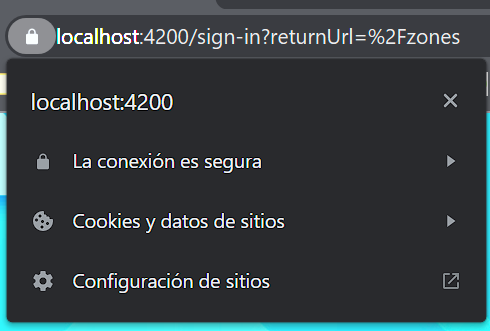
\includegraphics[width=.5\textwidth]{./Figures/Frontend certificados TLS.png}
	\caption{Certificados TLS aplicados.}
	\label{fig:certificadosTLSDelFrontendAplicados}
\end{figure} 

Se utilizó Lighthouse para realizar una auditoría del \emph{frontend}, los aspectos evaluados son: rendimiento, accesibilidad, mejores prácticas, SEO y un chequeo del tipo de aplicación: si es PWA se evalúa su implementación, caso contrario se restan puntos al resultado de la auditoría. La herramienta fue aplicada a las tres pantallas más demandantes del sistema: \emph{dashboard} de una zona, listado de zonas y listado de notificaciones.

En la figura \ref{fig:lighthouseDashboardZona} se presenta el resultado de la auditoría realizada sobre la pantalla de \emph{dashboard} de una zona.

\begin{figure}[H]
	\centering
	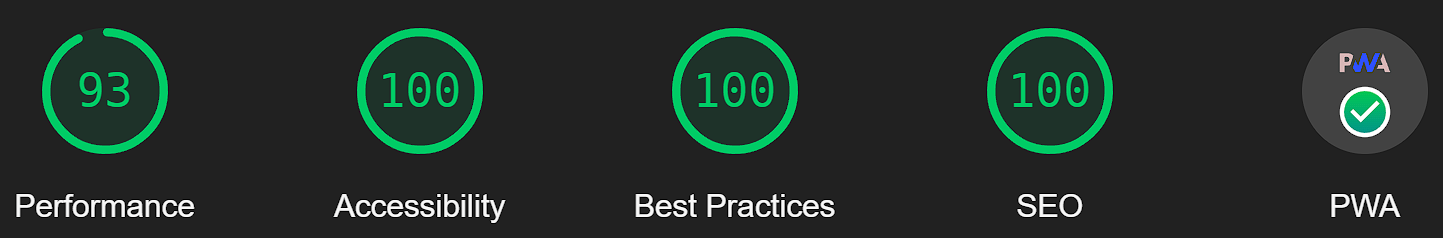
\includegraphics[width=.9\textwidth]{./Figures/Lighthouse dashboard.png}
	\caption{Auditoría realizada sobre la pantalla de \emph{dashboard} de una zona}
	\label{fig:lighthouseDashboardZona}
\end{figure}

En la figura \ref{fig:lighthouseListadoZonas} se presenta el resultado de la auditoría realizada sobre la pantalla de listado de zonas.

\begin{figure}[H]
	\centering
	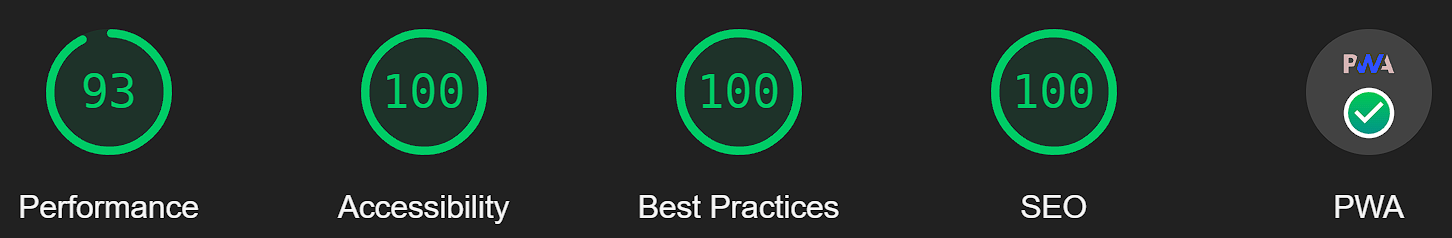
\includegraphics[width=.9\textwidth]{./Figures/Lighthouse zonas.png}
	\caption{Auditoría realizada sobre la pantalla de listado de zonas}
	\label{fig:lighthouseListadoZonas}
\end{figure}

En la figura \ref{fig:lighthouseListadoZonas} se presenta el resultado de la auditoría realizada sobre la pantalla de listado de notificaciones.

\begin{figure}[H]
	\centering
	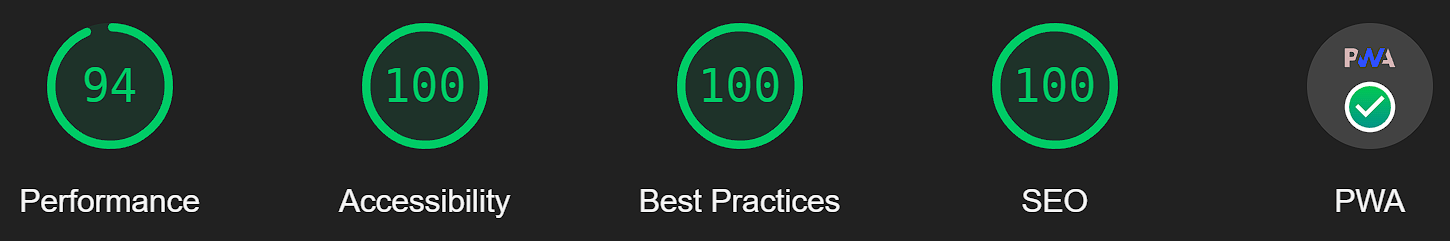
\includegraphics[width=.9\textwidth]{./Figures/Lighthouse notificaciones.png}
	\caption{Auditoría realizada sobre la pantalla de listado de notificaciones}
	\label{fig:lighthouseListadoZonas}
\end{figure}

Las tres auditorías realizadas obtuvieron la puntuación máxima en todas las categorías, excepto en rendimiento. Para alcanzar la máxima puntuación en rendimiento, es necesario reducir o eliminar el código JavaScript que no se utiliza en la aplicación.
 
\section{Pruebas del \emph{backend}}

Para probar el \textit{backend} se decidió utilizar una batería de pruebas unitarias creadas con Jest. Estás fueron completamente automatizadas para garantizar y asegurar la calidad de código. Se realizaron 78 pruebas unitarias para lograr un 100\% de cobertura de código. 

En la figuras \ref{fig:unitTestingBackend1} y \ref{fig:unitTestingBackend2} se visualiza el proceso de ejecución de las pruebas unitarias con Jest.

\begin{figure}[H]
	\centering
	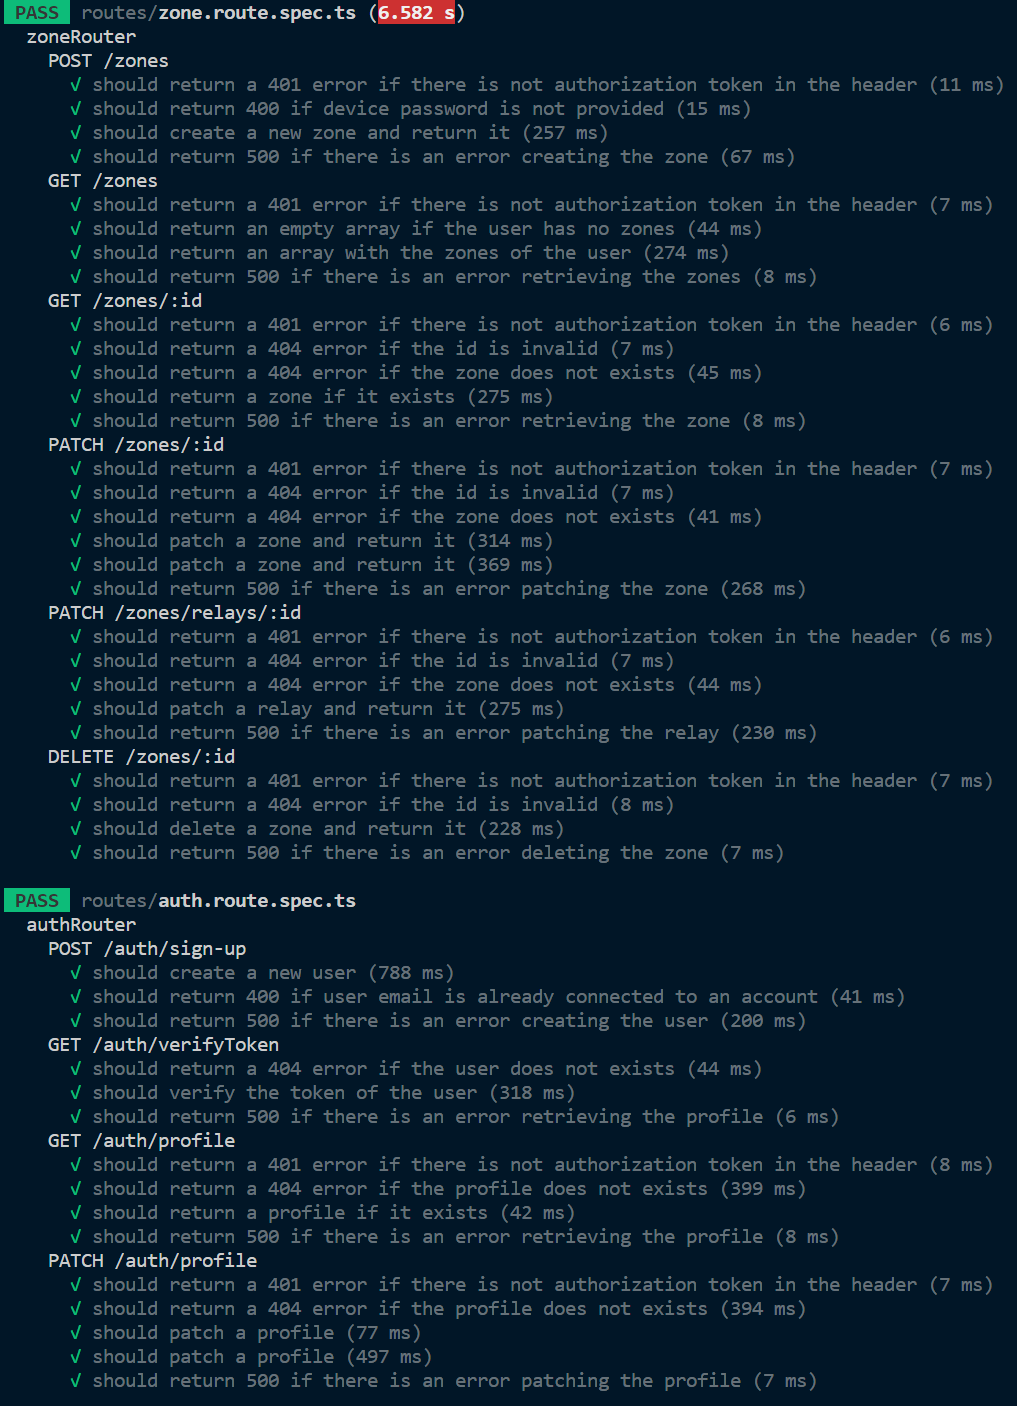
\includegraphics[width=.9\textwidth]{./Figures/Backend unit testing.png}
	\caption{Pruebas unitarias parte 1 de 2.}
	\label{fig:unitTestingBackend1}
\end{figure}

\begin{figure}[H]
	\centering
	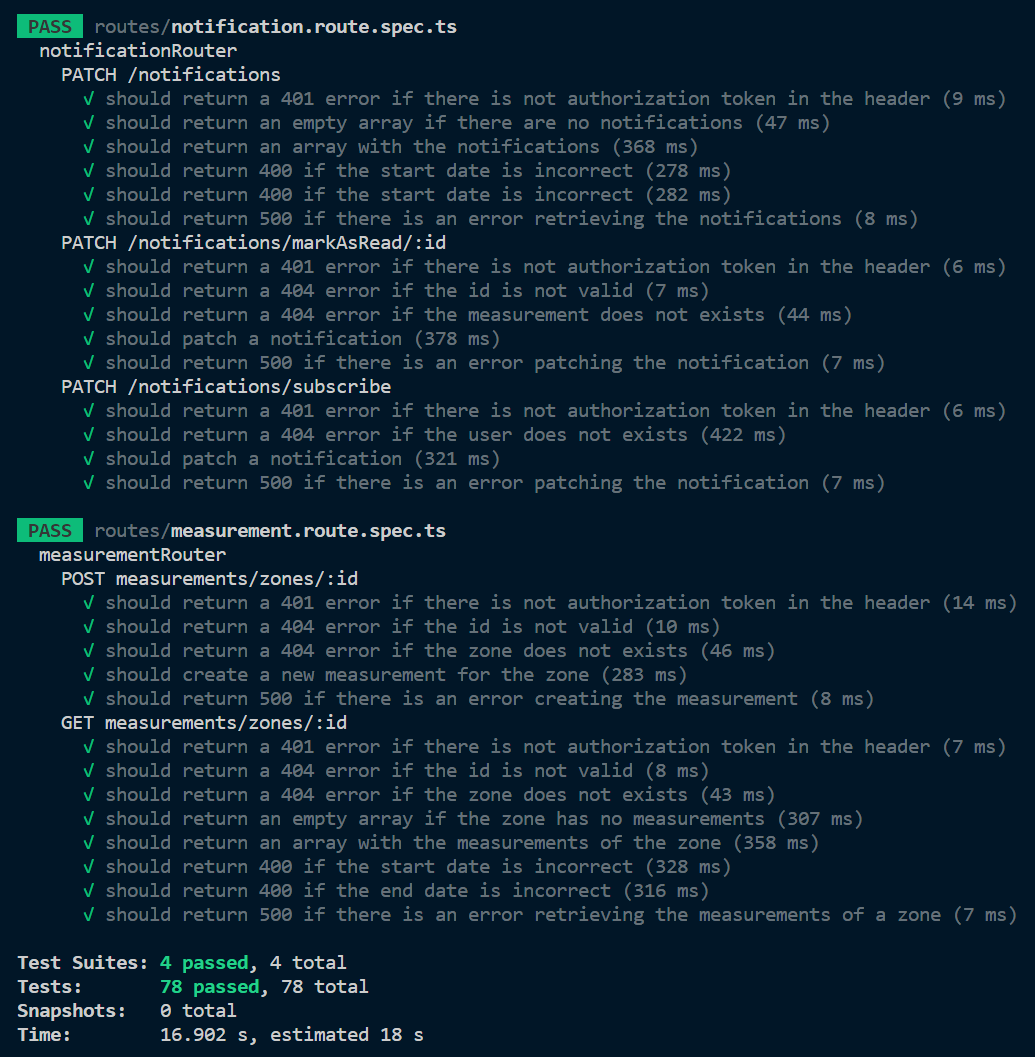
\includegraphics[width=.9\textwidth]{./Figures/Backend unit testing 2.png}
	\caption{Pruebas unitarias parte 2 de 2.}
	\label{fig:unitTestingBackend2}
\end{figure}


En la figura \ref{fig:codeCoverageBackend} se visualiza la cobertura de código del \emph{backend}.

\begin{figure}[H]
	\centering
	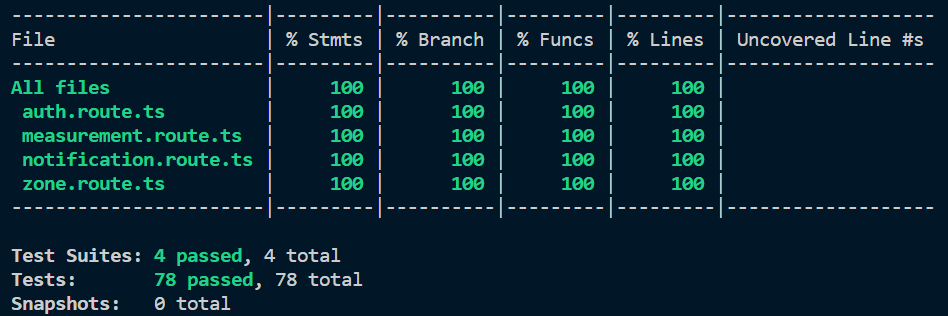
\includegraphics[width=.9\textwidth]{./Figures/Backend code coverage.png}
	\caption{Cobertura de código.}
	\label{fig:codeCoverageBackend}
\end{figure}

A modo de ejemplo, se presenta en el código \ref{cod:unitTestBackend} la prueba unitaria del \emph{endpoint} \textit{/zones}. En las líneas 2, 9, 19 y 31 se crean los casos de prueba. En las línea 3 a 6 se simula una \emph{request} al \emph{endpoint} sin haber configurado el \textit{authorization header}, además se valida que el código de la respuesta sea 401. En las líneas 10 a 16 se simula una \emph{request} al \emph{endpoint}, además se valida que el código de la respuesta sea 200 y que el \textit{body} sea una lista vacía. En la línea 20 se crea una zona. En las líneas 21 a 25 se simula una \emph{request} al \emph{endpoint} y se valida que el código de respuesta sea 200. En la línea 27 se elimina la zona creada. En la línea 28 se valida que el \textit{body} de la respuesta sea una lista con la zona creada. En las líneas  32 a 34 se crea un \emph{mock} sobre un método del ORM Mongoose para simular un error cuando se ejecute. En las líneas 36 a 40 se simula una \emph{request} al \emph{endpoint} y se valida que el código de respuesta sea 500.

\begin{lstlisting}[label=cod:unitTestBackend,caption=Prueba unitaria del \emph{endpoint /zones}]
describe("GET /zones", () => {
  it("should return a 401 error if there is not authorization token in the header", async () => {
    const response = await request(app)
      .get("/api/zones")
      .trustLocalhost()
      .expect(401);
  });

  it("should return an empty array if the user has no zones", async () => {
    const response = await request(app)
      .get("/api/zones")
      .trustLocalhost()
      .set("Authorization", `Bearer ${token}`)
      .expect(200);

    expect(response.body).toEqual([]);
   });

  it("should return an array with the zones of the user", async () => {
    await createZone();
    const response = await request(app)
      .get("/api/zones")
      .trustLocalhost()
      .set("Authorization", `Bearer ${token}`)
      .expect(200);

    await deleteZone();
    expect(response.body).toEqual([zone]);
  });

  it("should return 500 if there is an error retrieving the zones", async () => {
    jest.spyOn(Zone, "find").mockImplementation(() => {
      throw new Error();
    });

    const response = await request(app)
      .get("/api/zones")
      .trustLocalhost()
      .set("Authorization", `Bearer ${token}`)
      .expect(500);

    jest.spyOn(Zone, "find").mockRestore();
    expect(response.statusCode).toEqual(500);
  });
});
\end{lstlisting} 

%\section{Pruebas del \emph{broker}}

%Con el objetivo de validar la conexión con certificados TLS al \emph{broker} MQTT se realizaron cuatro pruebas manuales:

%\begin{itemize}
	%\item Caso de prueba uno: intento de conexión sin credenciales ni certificados.
	%\item Caso de prueba uno: intento de conexión con credenciales pero sin certificados.
	%\item Caso de prueba tres: intento de conexión con credenciales y certificados inválidos.
	%\item Caso de prueba cuatro: intento de conexión con credenciales y certificados válidos.
%\end{itemize}

\section{Prueba final de integración}

Se realizó una prueba final de integración para verificar el correcto funcionamiento del sistema.

En la figura \ref{fig:diagramaBancoDePruebas} se visualiza un diagrama del banco de pruebas con los componentes y relaciones que lo forman.

\begin{figure}[H]
	\centering
	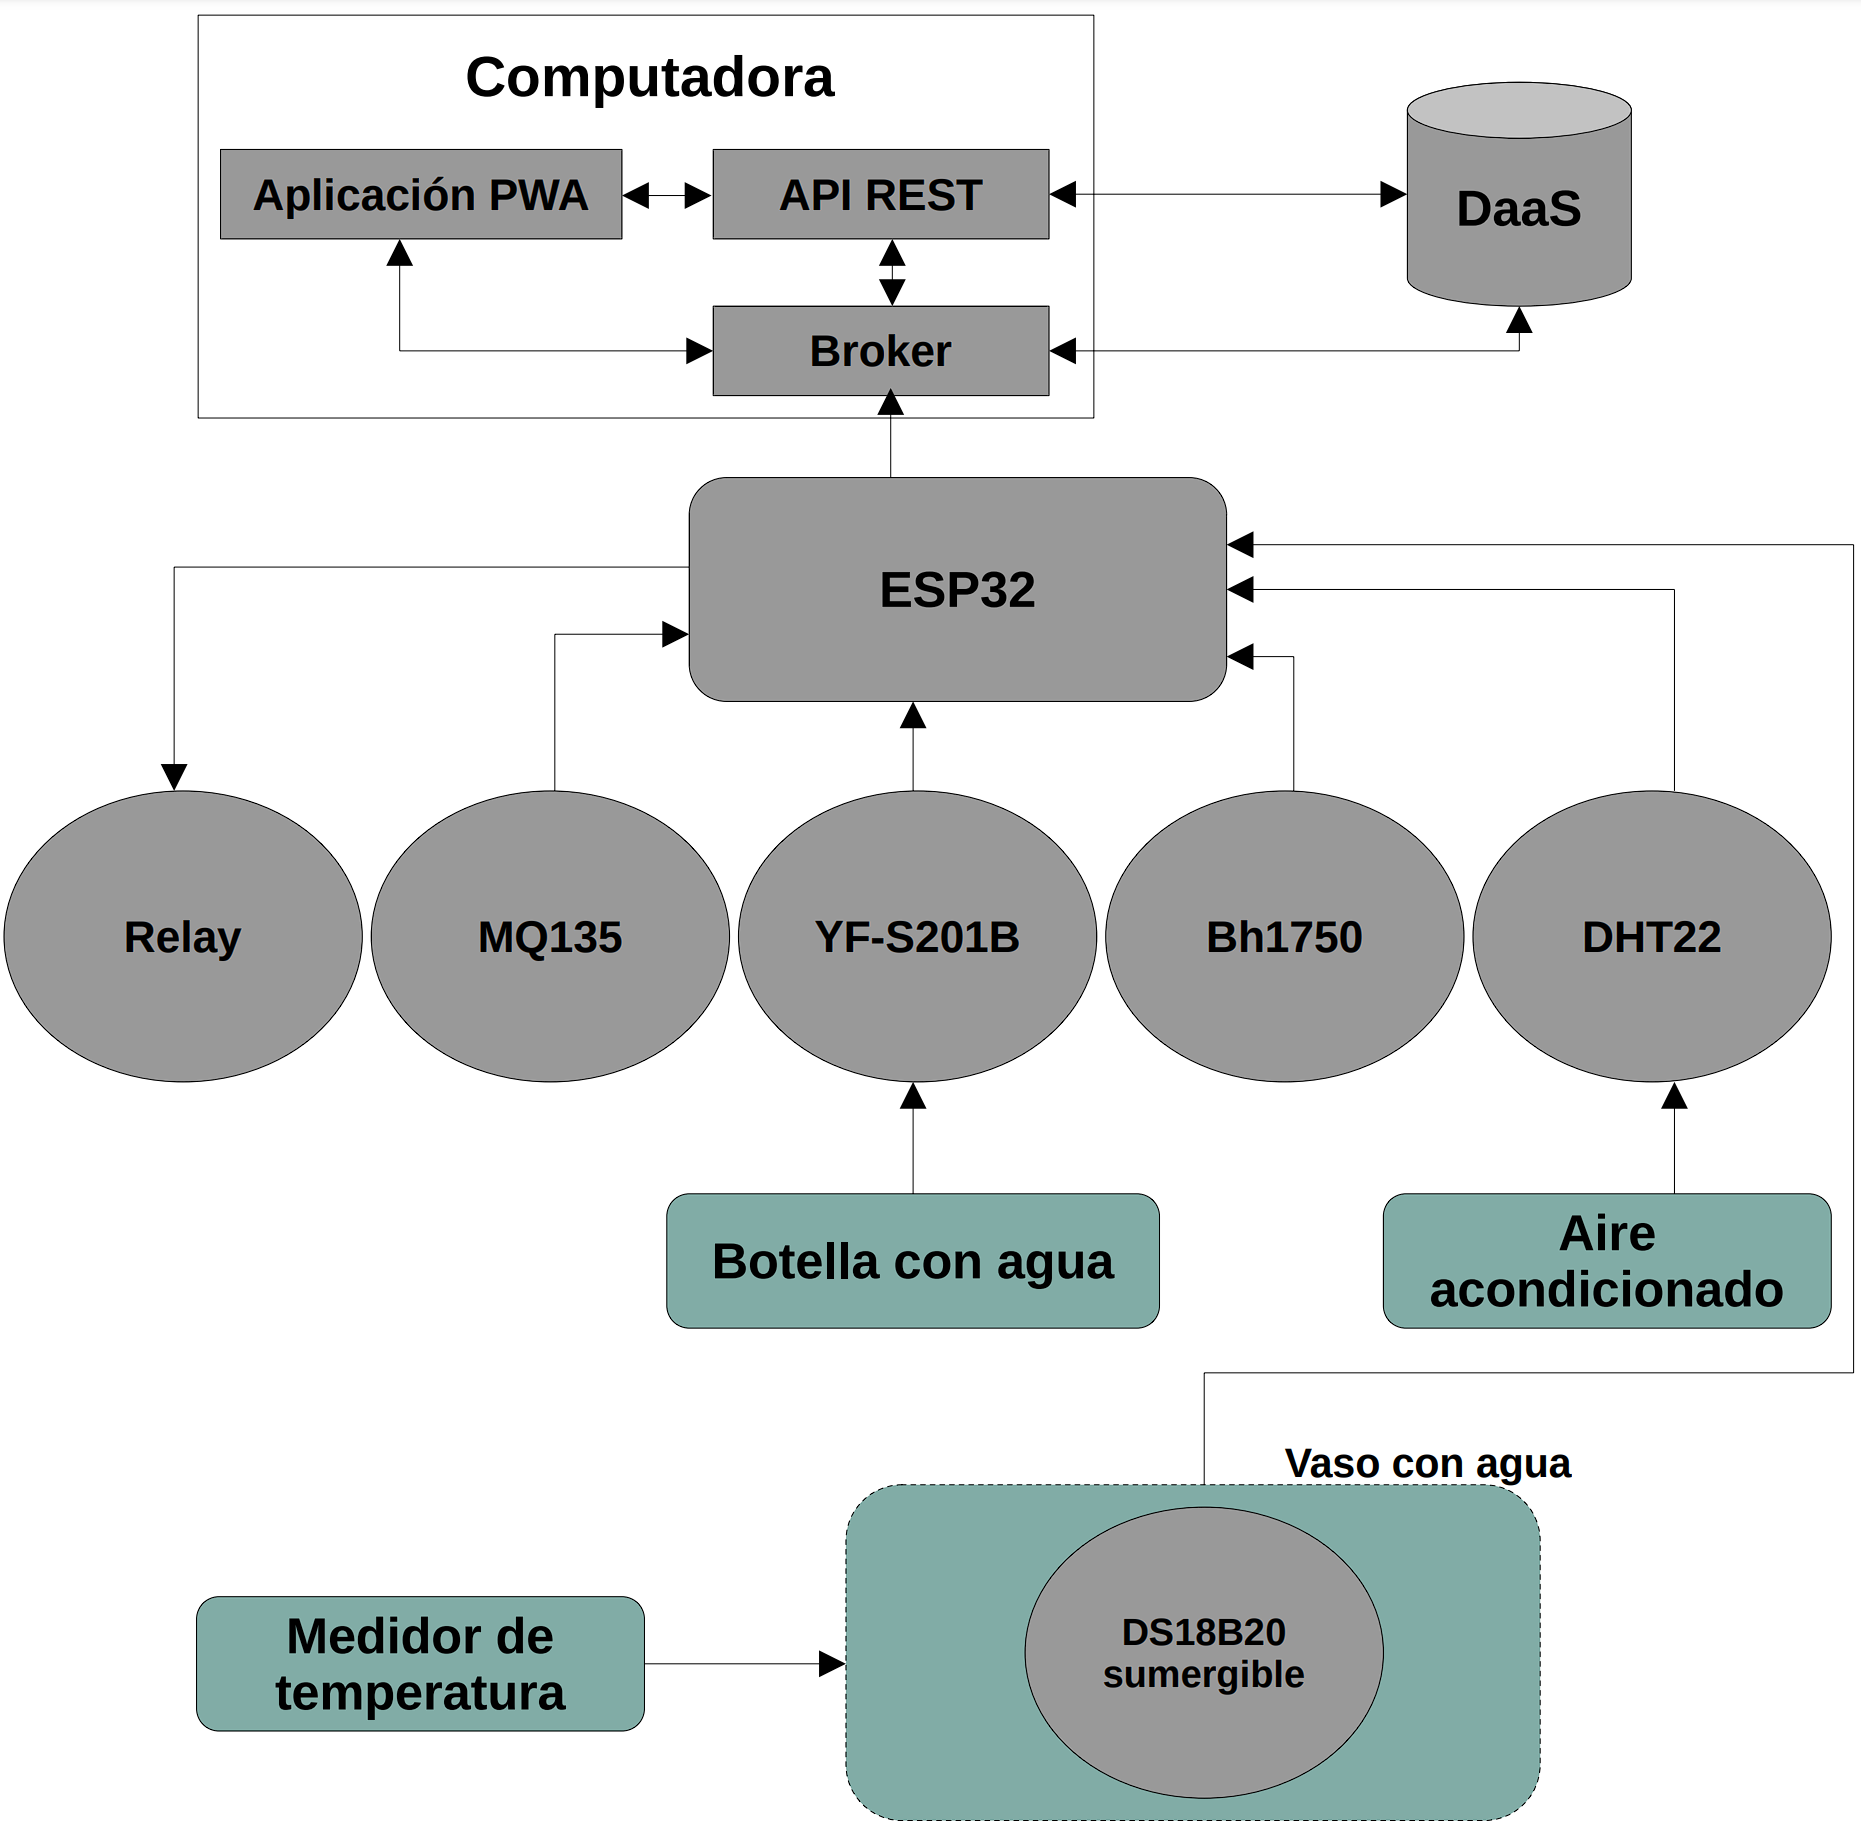
\includegraphics[width=.9\textwidth]{./Figures/Diagrama del banco de pruebas v2.png}
	\caption{Diagrama del banco de pruebas.}
	\label{fig:diagramaBancoDePruebas}
\end{figure}

Los pasos previos de configuración de la prueba consistieron en:

\begin{itemize}
	\item Inicializar el \textit{backend} y el \textit{broker} por medio del comando npm run dev. En la figura \ref{fig:inicializacionBackendIntegracion} se visualiza el resultado de la ejecución del comando.

\begin{figure}[H]
	\centering
	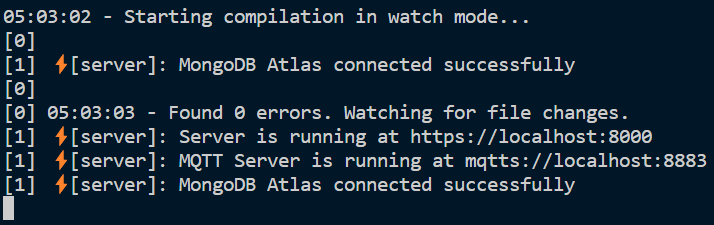
\includegraphics[width=.9\textwidth]{./Figures/Backend inicializacion.png}
	\caption{Inicialización del \emph{backend}.}
	\label{fig:inicializacionBackendIntegracion}
\end{figure}

	\item Inicializar el \textit{frontend} por medio del comando npm run lite-server. En la figura \ref{fig:inicializacionFrontendIntegracion} se visualiza el resultado de la ejecución del comando.

\begin{figure}[H]
	\centering
	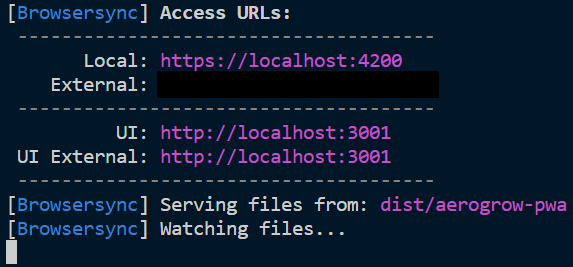
\includegraphics[width=.9\textwidth]{./Figures/Frontend inicializacion.png}
	\caption{Inicialización del \emph{frontend}.}
	\label{fig:inicializacionFrontendIntegracion}
\end{figure}

	\item Iniciar sesión en el sistema con una cuenta creada previamente.
	\item Crear una nueva zona de cultivo que tenga un \textit{relay} y dos alarmas. La primera alarma se dispara si la temperatura del ambiente es diferente a 1 °C y tiene una acción asociada que activa el \textit{relay} si la alarma se dispara por una temperatura mayor a 1 °C. La segunda alarma se dispara si la temperatura del líquido es menor a 1 °C o mayor a 2 °C. En las figuras \ref{fig:crearNuevaZonaIntegracion} y \ref{fig:listadoDeZonasIntegracion} se visualiza el proceso de creación de la zona.
	
	\begin{figure}[H]
	\centering
	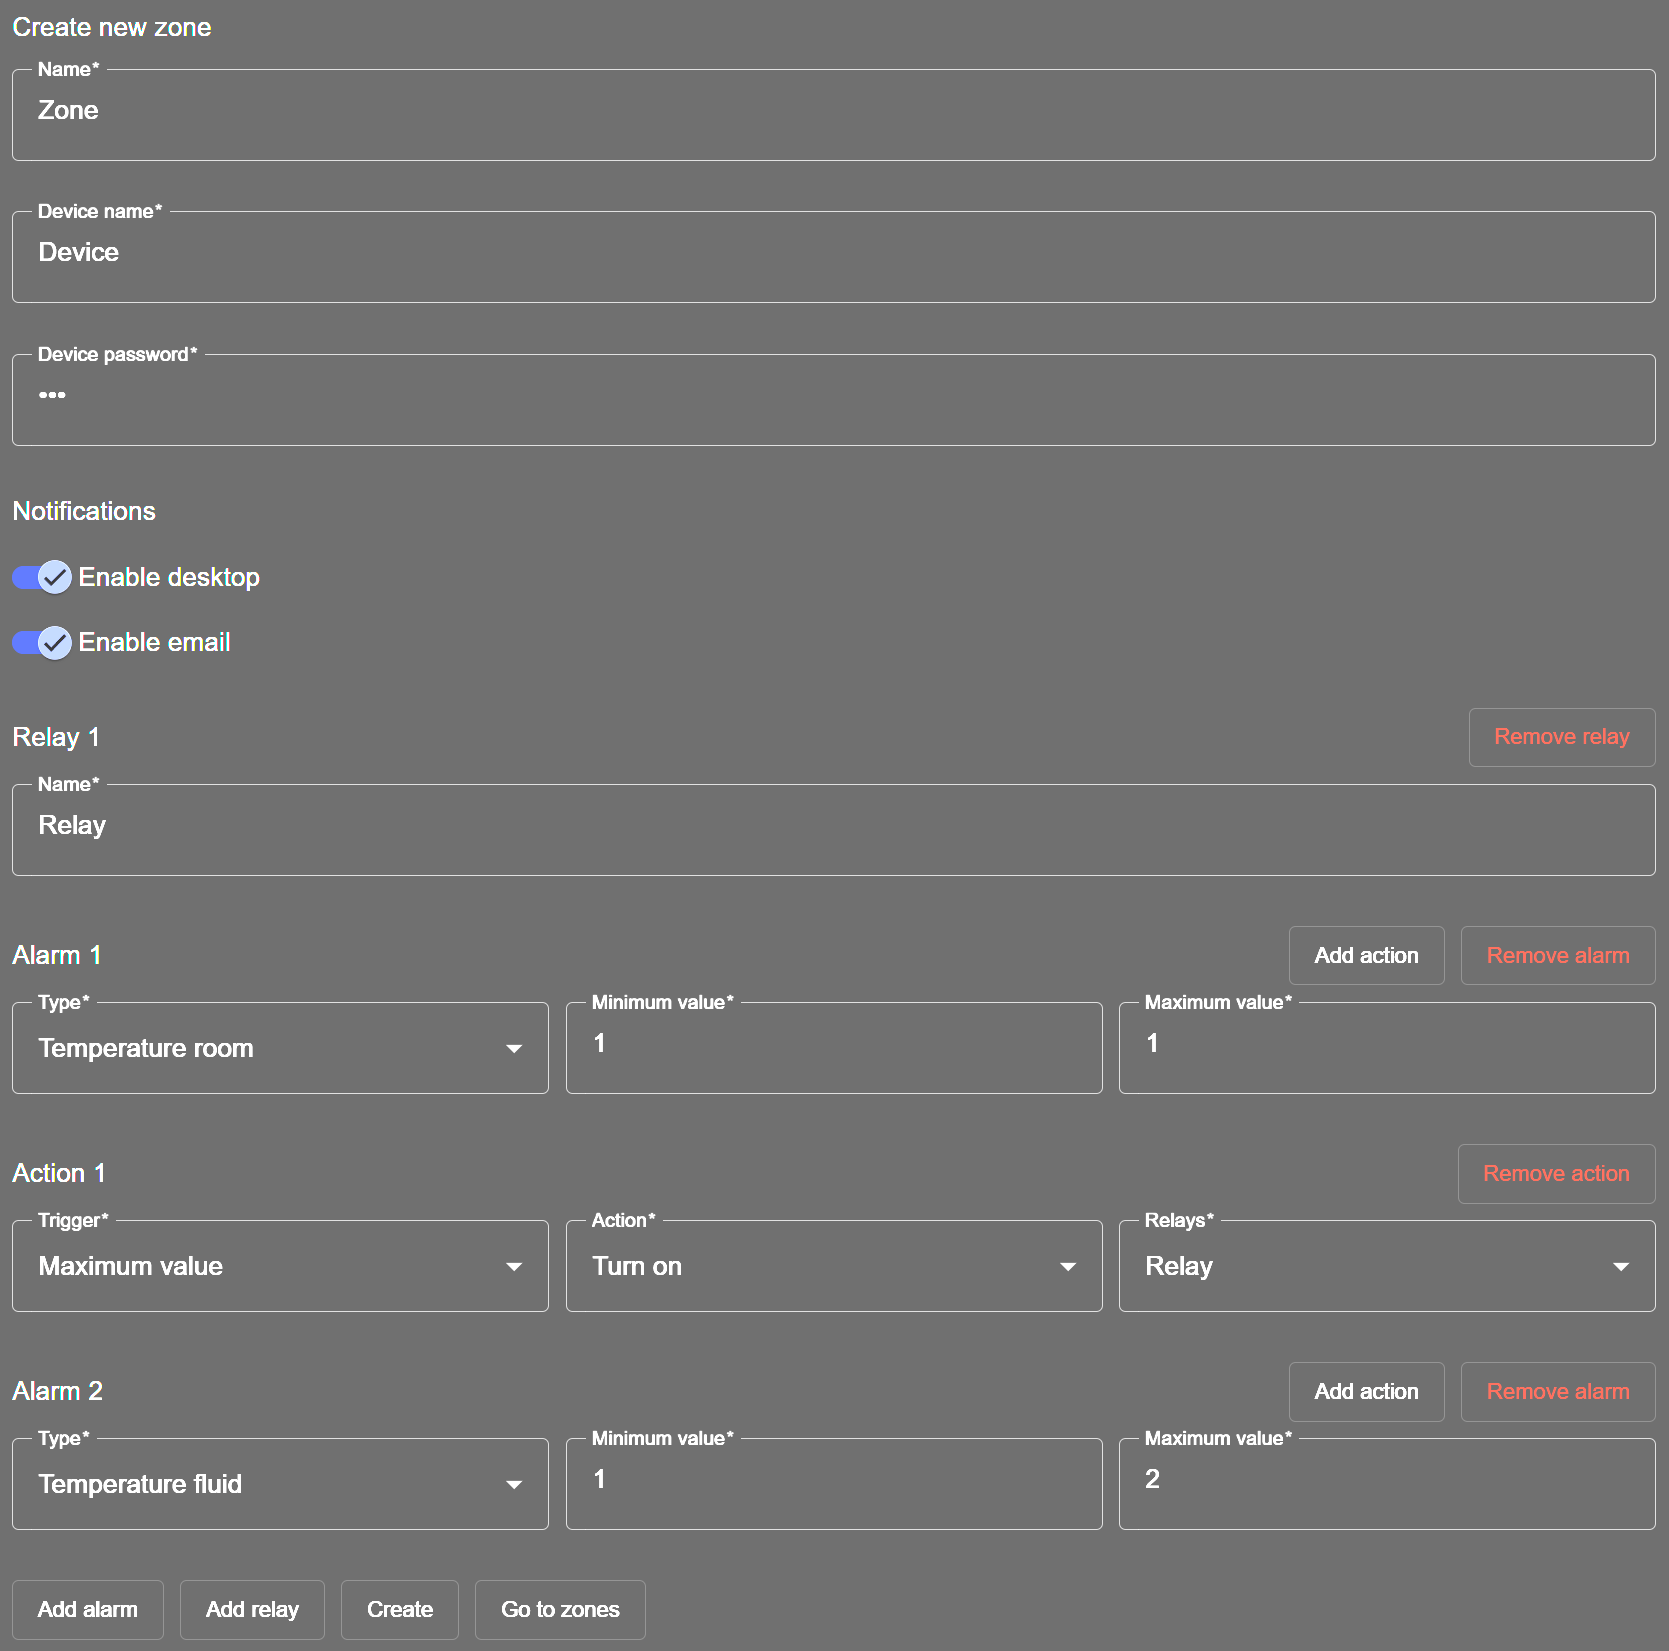
\includegraphics[width=.9\textwidth]{./Figures/Frontend crear nueva zona.png}
	\caption{Pantalla de creación de una zona.}
	\label{fig:crearNuevaZonaIntegracion}
\end{figure}

\begin{figure}[H]
	\centering
	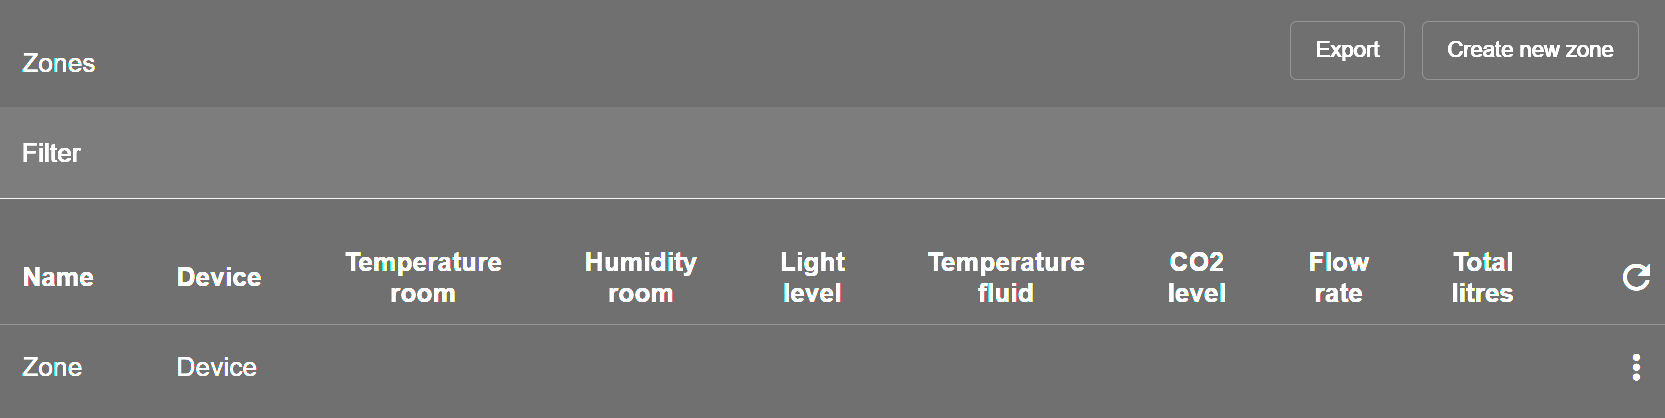
\includegraphics[width=.9\textwidth]{./Figures/Frontend nueva zona creada.png}
	\caption{Pantalla de listado de zonas.}
	\label{fig:listadoDeZonasIntegracion}
\end{figure}
	
	\item Conectar y configurar el \textit{software} del microcontrolador con las credenciales de la zona. En la figura \ref{fig:configuracionMicrocontroladorConfiguradoCredenciales} se presenta la configuración de credenciales en el microcontrolador.
	
\begin{figure}[H]
	\centering
	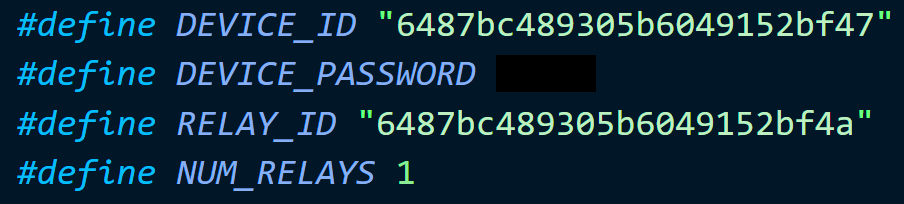
\includegraphics[width=.9\textwidth]{./Figures/Microcontrolador configuracion credenciales.png}
	\caption{Configuración de credenciales en el microcontrolador.}
	\label{fig:configuracionMicrocontroladorConfiguradoCredenciales}
\end{figure}

	\item Programar el microcontrolador con las nuevas credenciales.

	\item Monitorear el microcontrolador. En la figura \ref{fig:microcontroladorMonitoreo} se observa una parte del proceso de monitoreo mediante la extensión PlatformIO.
	
\begin{figure}[H]
	\centering
	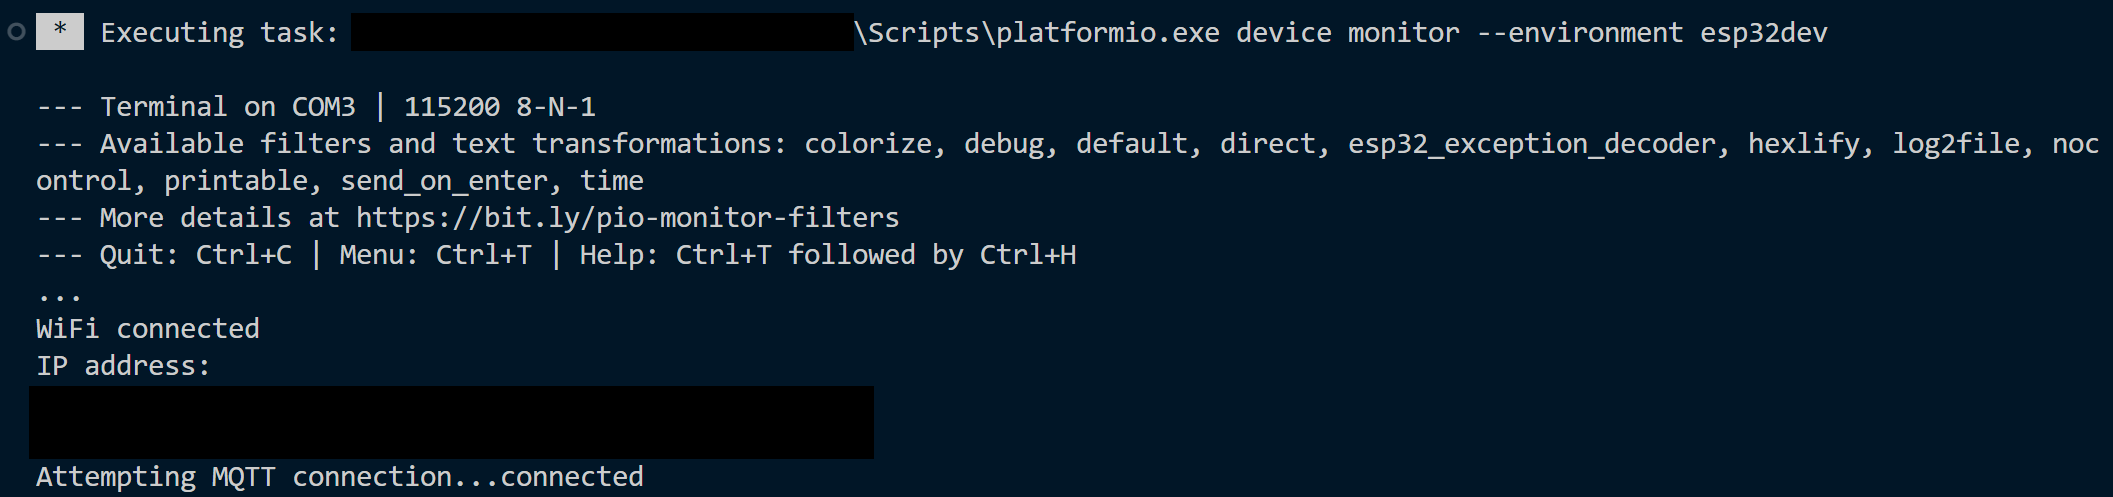
\includegraphics[width=.9\textwidth]{./Figures/Microcontrolador monitoreo.png}
	\caption{Monitoreo del microcontrolador.}
	\label{fig:microcontroladorMonitoreo}
\end{figure}
\end{itemize}

Para asegurar que se active la primera alarma, se colocó el sensor DHT22 en un ambiente con un aire acondicionado \citep{WEBSITE:BGHR410A} encendido en una temperatura de 24 °C por 30 minutos. 

Para asegurar que se dispare la segunda alarma, se colocó el sensor DS18B20 en un recipiente con agua previamente validada con un medidor externo \citep{WEBSITE:TP101} para asegurar que su temperatura sea de al menos 20 °C. 

Para que todos los sensores reporten valores al microcontrolador, se ingresó agua manualmente al sensor YF-S201B.

En las figuras \ref{fig:frontendListadoMedicionesPruebaDeIntegracion} y \ref{fig:frontendDashboardDeZonaPruebaDeIntegracion} se observa la pantalla de \textit{dashboard} de la zona con la medición registrada y el \textit{relay} activo. 

\begin{figure}[H]
	\centering
	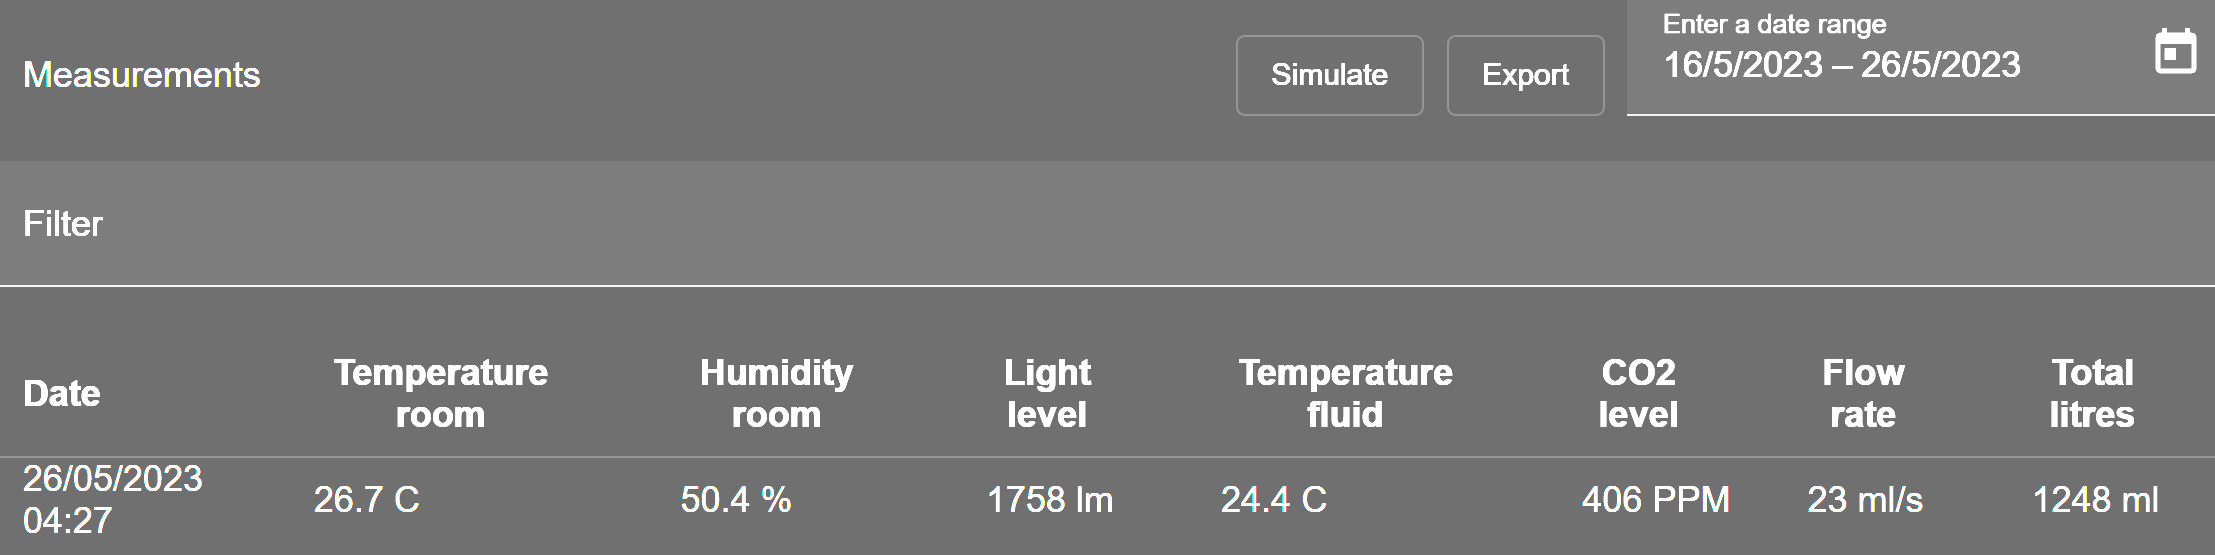
\includegraphics[width=.9\textwidth]{./Figures/Frontend listado de mediciones prueba de integracion.png}
	\caption{Listado de mediciones en vista de \textit{dashboard}.}
	\label{fig:frontendListadoMedicionesPruebaDeIntegracion}
\end{figure}

\begin{figure}[H]
	\centering
	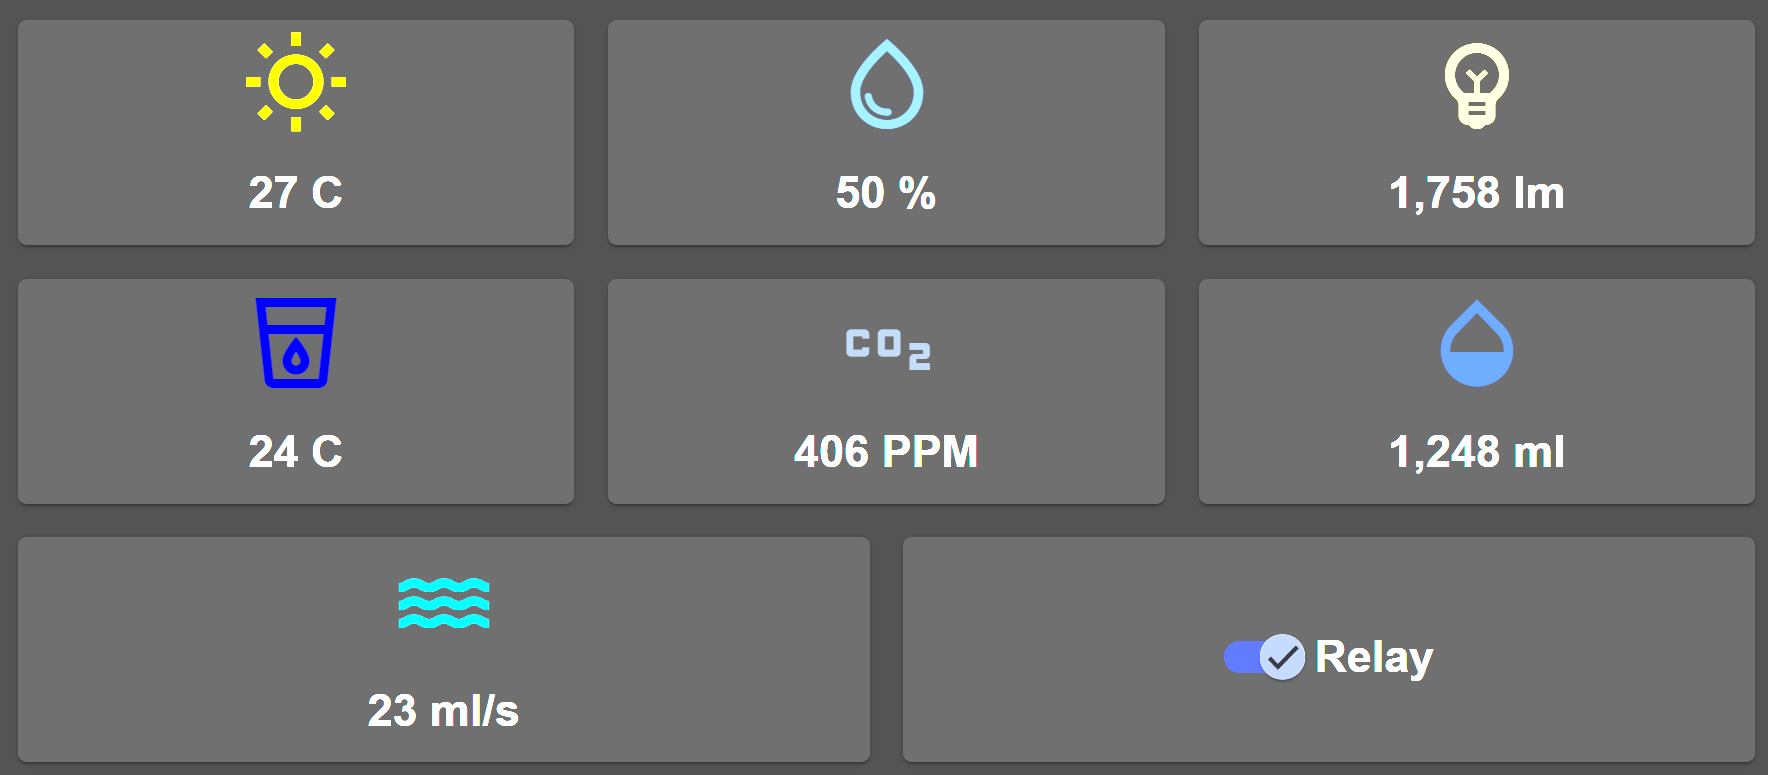
\includegraphics[width=.9\textwidth]{./Figures/Frontend dashboard de zona cards prueba de integracion.png}
	\caption{\textit{Cards} en vista de \textit{dashboard}.}
	\label{fig:frontendDashboardDeZonaPruebaDeIntegracion}
\end{figure}

En las figuras \ref{fig:frontendListadoDeNotificacionesPruebaDeIntegracion}, \ref{fig:notificacionEmailPruebaDeIntegracion} y \ref{fig:notificacionDesktopruebaDeIntegracion} se presentan las notificaciones enviadas por el sistema al activarse la alarma.

\begin{figure}[H]
	\centering
	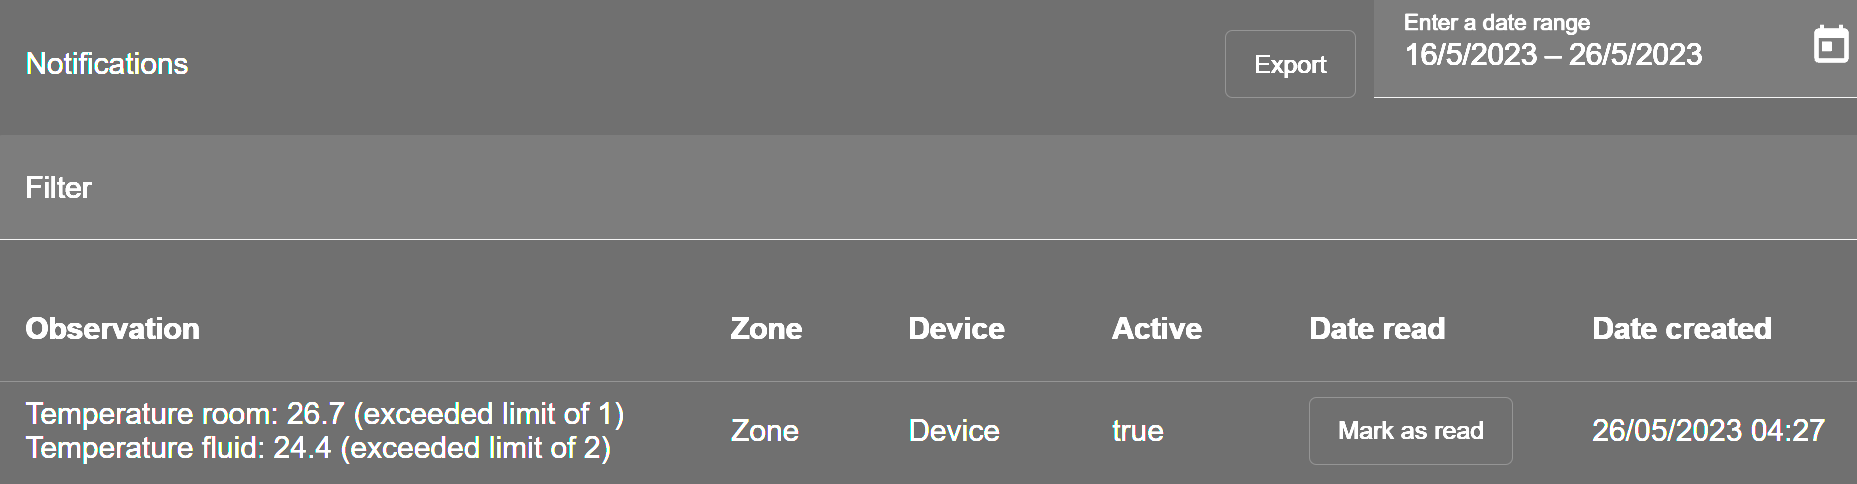
\includegraphics[width=.9\textwidth]{./Figures/Frontend listado de notificaciones prueba de integracion.png}
	\caption{Pantalla de listado de notificaciones.}
	\label{fig:frontendListadoDeNotificacionesPruebaDeIntegracion}
\end{figure}

\begin{figure}[H]
	\centering
	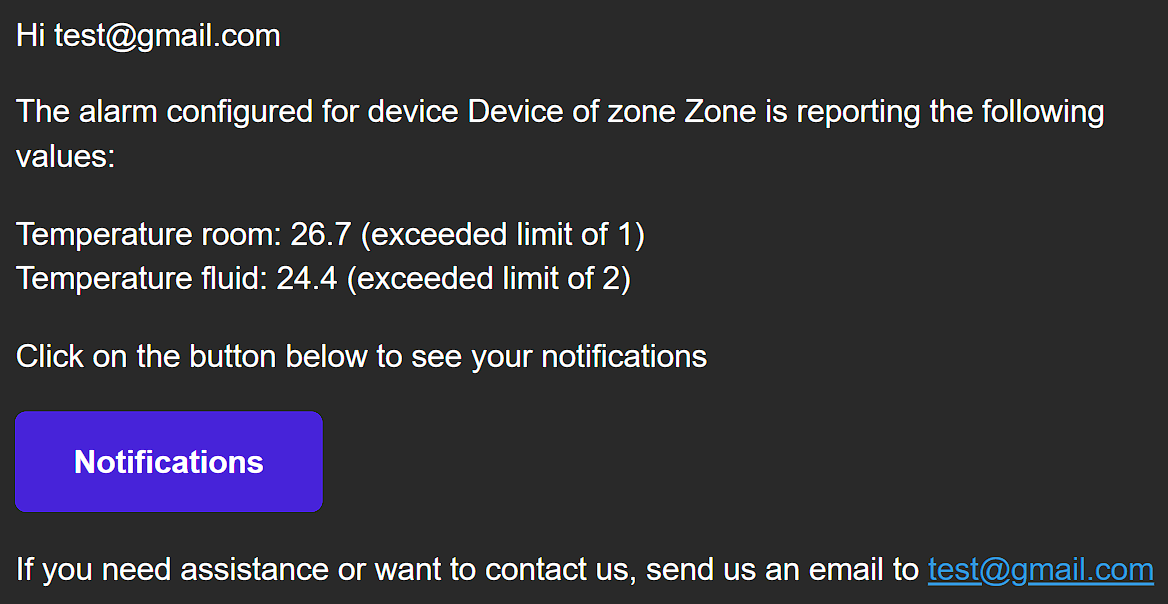
\includegraphics[width=.8\textwidth]{./Figures/Notificacion email prueba de integracion.png}
	\caption{\textit{Email} enviado por el sistema.}
	\label{fig:notificacionEmailPruebaDeIntegracion}
\end{figure}

\begin{figure}[H]
	\centering
	
\includegraphics[width=.5\textwidth]{./Figures/Notificacion desktop prueba de integracion.png}
	\caption{Notificación \textit{push} enviada por el sistema.}
	\label{fig:notificacionDesktopruebaDeIntegracion}
\end{figure}

\section{Comparación con el estado del arte}

En la tabla \ref{tab:comparativaTrabajoSolucionesNacionalesInternacionales} se presenta la comparación de las características y funcionalidades entre los sistemas comerciales encontrados en el mercado nacional e internacional y el trabajo realizado llamado Aerogrow.

\begin{table}[H]
	\centering
	\caption[Comparativa entre soluciones comerciales similares y el trabajo realizado]{Comparativa entre soluciones comerciales similares y el trabajo realizado.}
	\begin{tabular}{l c c c}    
		\toprule
		\textbf{Funcionalidad} & \textbf{Smartcultiva} & \textbf{My Autogrow} & \textbf{Aerogrow}\\
		\midrule
		MQTT & Sí & Sí & Sí \\
		Sistema de alertas & Sí & Sí & Sí\\
		Acciones automatizadas & Sí & No & Sí\\
		Notificaciones \emph{push} & No & No & Sí\\
		Notificaciones \textit{email} & Sí & Sí & Sí\\
		\shortstack{Accionamiento de \\ dispositivos externos} & Sí & No & Sí\\
		Escalabilidad en sensores & Limitado & Limitado & Alta\\
		Tipo de aplicación & Móvil y web & Web & PWA\\
		\bottomrule
		\hline
	\end{tabular}
	\label{tab:comparativaTrabajoSolucionesNacionalesInternacionales}
\end{table}

En la tabla \ref{tab:comparativaTrabajoSolucionesPublicacionesCientificas} se presenta la comparación de las características y funcionalidades entre los sistemas encontrados en publicaciones científicas y el trabajo realizado.

\begin{table}[H]
	\centering
	\caption[Comparativa entre soluciones similares encontradas en publicaciones científicas y el trabajo realizado]{Comparativa entre soluciones similares encontradas en publicaciones científicas y el trabajo realizado.}
	\begin{tabular}{l c c c}    
		\toprule 
		\textbf{Funcionalidad} & \textbf{\textit{Monitoring Soil (...)}} & \textbf{\textit{A Smart (...)}}  & \textbf{Aerogrow}\\
		\midrule
		MQTT & Sí & No  & Sí\\
		LoRa & Sí & Sí  & No\\
		Sistema de alertas & No & Sí & Sí\\
		\shortstack{Acciones \\ automatizadas} & No & No & Sí\\
		Notificaciones \emph{push} & No & No & Sí\\
		Notificaciones \textit{email} & No & Sí & Sí\\
		\shortstack{Accionamiento de \\ dispositivos externos} & No & No & Sí\\
		\shortstack{Escalabilidad en \\ sensores} & Media & Media & Alta\\
		Tipo de aplicación & Web & Web & PWA\\
		\bottomrule
		\hline
	\end{tabular}
	\label{tab:comparativaTrabajoSolucionesPublicacionesCientificas}
\end{table}

De acuerdo a la comparación realizada, el trabajo elaborado se destaca por permitir recibir notificaciones \emph{push} y por la escalabilidad para añadir nuevos sensores. Sin embargo, se debe tener en cuenta los siguientes factores:

\begin{itemize}
\item Smartcultiva y este trabajo son las únicas soluciones que permiten crear acciones automatizadas cuando se activa una alerta. 
\item Smartcultiva y este trabajo son las únicas soluciones que permiten el accionamiento de dispositivos externos.
\item Las dos publicaciones científicas soportan el uso del protocolo LoRa.
\end{itemize}